\section{Introduction}

Many programmers develop code by interleaving opportunistic information foraging with writing code~\cite{brandt_two_2009,brandt_example-centric_2010}.
When learning about unfamiliar technologies, programmers often start by searching for tutorial web sites.
Instead of examining the prose, they experiment with code examples, using source code from the pages to support learning by doing~\cite{brandt_two_2009}.
However, programmers of all backgrounds~\cite{duala-ekoko_asking_2012,dorn_lost_2013,dorn_learning_2010} struggle to leverage web documentation to solve programming problems.

One source of confusion is that authors write teaching materials with a certain audience in mind.
This target audience determines what  information is included, and what is omitted.
For example, an author of a tutorial on web scraping may expect readers to be familiar with Python, CSS selectors, regular expressions, and threads.
However, the actual audience may have different skills.
As a result, \shortchange{answers on Q\&A sites like StackOverflow may have insufficient  explanation~\cite{nasehi_what_2012}}, and tutorial-style blogs may lack  scaffolding for readers seeking clarification on unfamiliar or complex syntax.

\begin{figure}[!t]
\centering{%
    \subfigure[A \gls{exp} of a CSS selector with an automatically generated natural language explanation and demonstration of an HTML element it matches.]{%
        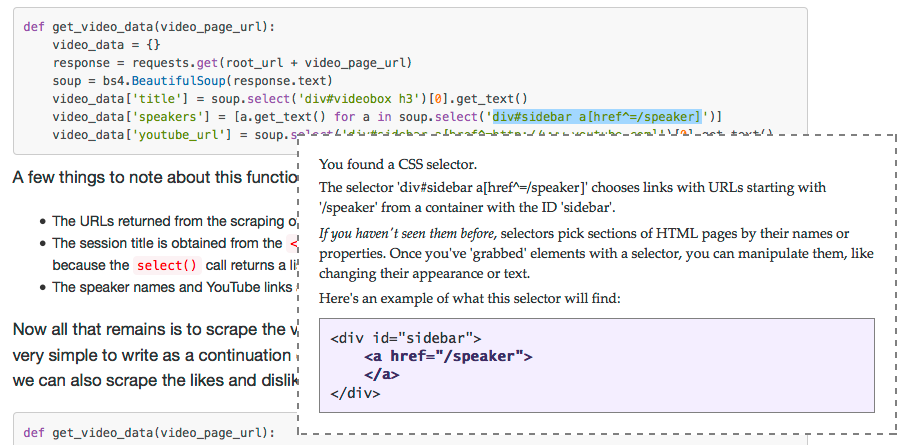
\includegraphics[width=\columnwidth]{figures/accelerator_css}\label{fig:accelerator_css}
    }
    \subfigure[A \gls{exp} describing the high-level intent and low-level argument values of a wget command.]{%
        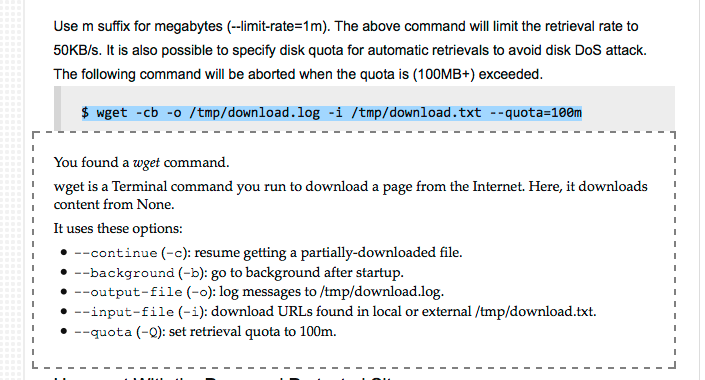
\includegraphics[width=\columnwidth]{figures/accelerator_wget}\label{fig:accelerator_wget}
    }
    \caption{%
    \Gls{name}-generated \glspl{exp} enable programmers to seek in-situ help when reading and adapting code found in online tutorials and Q\&As.
    Programmers select the code they want clarification about, and view natural language descriptions and demonstrations of what the code does.
    }\label{fig:accelerators}
}
\end{figure}

\if 0
\begin{changes}
One of the attributes of recognized answers on StackOverflow, according to Nasehi et al.~\cite{nasehi_what_2012}, is step-by-step solutions.
A step-by-step solution is presented in a detailed and ordered fashion, in a simple way, in a way that's familiar to the questioner or friendly to newcomers.
Answers with this attribute sometimes provide a simulation of what the code does, or describe multiple elements needed to perform a single programming task. \if 0
Three common attributes of low-vote answers on StackOverflow (lack of explanation, in addition to lack of code and shortcomings of solution).
This implies that some code examples could be more valuable to programmers looking for online inspiration if their explanations were complete and at the appropriate level of detail~\cite{nasehi_what_2012}.
\fi
The routines we develop here enable step-by-step explanations and simulations of existing code to add value to existing code examples.
\end{changes}
\fi

To provide the missing scaffolding for unexplained code in tutorials, Q\&As, and other online programming help, we propose routines called \emph{\Glspl{name}} that produce context-relevant, on-demand descriptions of code for these embedded languages.
\Glspl{name} automatically find pieces of code in web pages and augment these with \glspl{exp}: such explanations are \emph{context-relevant}, describing only the syntactic elements that are present and important within a snippet, using domain-specific terms.
% In comparison to getting-started guides and reference documentation, \Glspl{name} minimize the amount of text programmers have to inspect to understand source code.
\if 0 
\begin{changes}
Such explanations begin to resemble the ``good answers'' from online Q\&A by providing detailed step-by-step solutions in a way that is familiar to the questioner~\cite{nasehi_what_2012}.
\end{changes}
\fi
They are also \emph{on-demand} --- they can describe confusing code found anywhere to provide just-in-time understanding.

\if 0
We draw on inspiration of layered documentation to justify our current work. \appachu{one liner to describe layered documentation}
Decades of research on technical communication provide best practices for writing usable documentation.
In the domain of software, minimalist instruction~\cite{carroll_nurnberg_1990} recommends enabling users to start immediately on realistic tasks, minimizing the necessary  reading and other passive activity, and supporting error recognition and recovery.
Farkas~\cite{farkas_layering_1998} introduces layered documentation as an extension to minimalist instruction that enables users from different backgrounds to benefit from the same documents by providing optional backup information for tasks like error recognition and correction.
\fi 
%
\begin{changes}
\Glspl{name} can be built to generate explanations for languages like CSS selectors, regular expressions, Unix commands (see Figure~\ref{fig:accelerators}), and other short one-liner languages. 
\end{changes}
\if 0 They are programmed to detect relevant code, parse it, and generate explanations and demonstrations of that code. 
\marti{This repeats a sentence in the abstract (or close to it.)} \fi
In our implementation, each language can be supported in several hundred lines of code.
Each one can be built as a standalone server, accessible by an addon in the programmer's browser to provide explanations of code anywhere on the web.
\if 0 With the \Glspl{name} that we build for CSS selectors, regular expressions and Unix commands, \fi \if 0 We show an expanse of domain-specific representations of code, from natural language to example HTML documents.\fi 

We make three main contributions.
First, we introduce a framework for building \Glspl{name}. \if 0 generators of explanations and demonstrations for domain-specific languages and Unix commands.\marti{This also repeats that language.} \fi
Second, we describe the processing pipeline, technical considerations, and design guidelines involved in building \Glspl{name}, providing details about our efforts to implement them for CSS selectors, regular expressions, and Unix commands.
Finally, we show through an in-lab study how \Gls{name}-generated \glspl{exp} can help programmers modify existing code without referring to external documentation.
